% Chapter 5: The Fourier Neural Operator: Spectral Theory and Convergence
% Part I of the book.

\chapter{The Fourier Neural Operator: Spectral Theory and Convergence}
\label{ch:part1-the-fourier-neural-operator-spectral-theor}
\label{sec:fno}
% -----------------------------------------------------------------------------

\chapref{ch:part1-operator-approximation-theory-and-universa} ends on an
existence result and says nothing about price. A neural operator built from a
pointwise lift, integral kernel layers, and a pointwise projection approximates
any continuous operator on a compact input set, provided the kernel
$\kappa_\ell(x,y,a(x),a(y))$ in \eqref{eq:fredholm_kernel} is free to depend on
both arguments and on the field itself. Discretized on $N$ quadrature nodes,
that freedom costs an $N \times N$ array per layer and a dense matrix-vector
product per application. A field on a $256 \times 256$ grid is
$N \approx 6.5 \times 10^4$ unknowns, so a single layer commits $4 \times 10^9$
kernel evaluations per input, and four layers make an existence proof into
arithmetic nobody pays for.

The \textbf{Fourier Neural Operator} (FNO)~\cite{li2021fourier} escapes the
\index{Fourier neural operator}
bottleneck by accepting a restriction rather than by inventing a faster dense
product. It requires the kernel to be \emph{stationary},
$\kappa(x,y)=\kappa(x-y)$, and the domain to be the periodic torus
$\mathbb{T}^d$. Both are modeling assumptions. They declare the medium
homogeneous and the boundary periodic, and they remove
the explicit input dependence that the generic kernel carries. The premise binds
the kernel of each layer; the network as a whole is freer --- the lifted
channels and the local bypass can partially disguise a mild inhomogeneity, as
the taxonomy of
\chapref{ch:part1-comparative-theoretical-taxonomy-of-archit} argues --- but it
cannot be wished away, and Section~\ref{sec:ch05-truncation} records what it
costs. In exchange,
translation invariance diagonalizes the operator. The complex exponentials are
eigenfunctions of every stationary convolution simultaneously, so the kernel
collapses from a function of $2d$ real variables to a function of one integer
index. A grid application then costs $\mathcal{O}(N \log N)$ with the fast
Fourier transform (FFT), against $\mathcal{O}(N^2)$ for the dense product.
\index{fast Fourier transform (FFT)}
\index{periodic domain (torus)}

This chapter develops that exchange at the level of rigor Part I requires. The
first section derives the multiplier representation and states plainly what
stationarity gives up. The second truncates the multiplier to a finite mode set
and assembles the continuum layer, comparing it term by term with the generic
construction. The third states the convergence theorem, works through its
proof, and reads the resulting rate off a computed figure. The reader should
arrive with the Fourier-series characterization of $H^s(\mathbb{T}^d)$ from
\chapref{ch:part1-function-spaces-duality-and-sobolev-regula}, the smoothing
examples of \chapref{ch:part1-partial-differential-equations-as-solution}, and
the architecture of \chapref{ch:part1-operator-approximation-theory-and-universa}.
Two warnings recur and are best stated at the outset: every bound below is an
upper bound whose constants the theory does not produce, and every statement
concerns the continuum layer rather than the discrete transform a training loop
evaluates. The second warning is the subject of
\chapref{ch:part1-discretization-invariance-and-continuum-li}.

% -----------------------------------------------------------------------------
\section{Fourier Multipliers and Stationary Convolutional Kernels}
\label{sec:ch05-multipliers}

The kernel layer \eqref{eq:fredholm_kernel} is deliberately general:
$\kappa_\ell$ may depend on the source point, the target point, and the input
field at both. That generality is what makes the universality theorem true and
what makes its discretization dense. The FNO surrenders the first two
dependencies at once. It works on the flat torus
$\mathbb{T}^d \cong [0,1)^d$ of
\chapref{ch:part1-function-spaces-duality-and-sobolev-regula} and assumes a
\textbf{stationary kernel}, a function of the separation alone, so that
substituting $\kappa(x,y) = \kappa(x-y)$ into \eqref{eq:fredholm_kernel} turns
the integral into a convolution on a compact abelian group:
\index{stationary kernel}
\index{translation-invariant kernel}
\index{convolution!on the torus}
\begin{equation}
  \label{eq:ch05-convolution}
  (\mathcal{K} v)(x) = \int_{\mathbb{T}^d} \kappa(x - y) v(y) \, dy = (\kappa * v)(x).
\end{equation}
For $\kappa, v \in L^2(\mathbb{T}^d)$ the integrand is integrable by
Cauchy--Schwarz, so \eqref{eq:ch05-convolution} is defined pointwise, and
Young's inequality on the torus upgrades it to a bounded function; when either
factor is smoother, the convolution inherits that smoothness.

The reason the restriction pays is that the Fourier basis diagonalizes every
stationary operator at once. Write the coefficients with the convention of
\chapref{ch:part1-function-spaces-duality-and-sobolev-regula},
$\hat{u}(k) = \int_{\mathbb{T}^d} u(x) e^{-2\pi i k \cdot x}\,dx$, so that
$u(x) = \sum_{k} \hat{u}(k) e^{2\pi i k \cdot x}$. For the exponential
$e_k(x) = e^{2\pi i k \cdot x}$ the change of variables $z = x - y$ gives
$(\kappa * e_k)(x) = e^{2\pi i k \cdot x} \int_{\mathbb{T}^d} \kappa(z)
e^{-2\pi i k \cdot z}\,dz = \hat{\kappa}(k)\, e_k(x)$. The exponentials are
eigenfunctions of \emph{all} such convolutions simultaneously, and the
eigenvalue attached to mode $k$ is precisely the $k$-th Fourier coefficient of
the kernel. Stated as an identity on coefficients, this is the convolution
theorem for Fourier series:
\index{convolution theorem}
\index{Fourier multiplier}
\begin{equation}
  \label{eq:ch05-convolution-theorem}
  \mathcal{F}(\kappa * v)(k) = \mathcal{F}(\kappa)(k) \cdot \mathcal{F}(v)(k) = \hat{\kappa}(k) \, \hat{v}(k), \quad k \in \mathbb{Z}^d.
\end{equation}

Equation \eqref{eq:ch05-convolution-theorem} is the entire computational
argument. An operator that mixed modes would need a matrix indexed by pairs of
frequencies; a stationary one needs a single sequence, and \eqref{eq:ch05-convolution-theorem}
shows the sequence is nothing but the kernel's own spectrum. Read the other
way, the same identity says exactly what has been given up: if $\kappa$ depends
on $x$ and $y$ separately, $\mathcal{K}$ scatters energy among modes and no
diagonal object represents it. Stationarity is a claim about the physics
--- homogeneous medium, no distinguished location, periodic boundary --- and a
learned filter on, say, a bounded domain with boundary layers either has to
disguise the inhomogeneity or hand it to another component.

Rather than parameterizing $\kappa(x-y)$ in physical space and integrating
numerically, the FNO parameterizes the multiplier directly. The hidden field
$v_\ell$ takes values in $\mathbb{R}^{d_v}$, so the multiplier is
matrix-valued:
\index{channel mixing}
\index{Fourier multiplier $R_\phi(k)$}
\begin{equation}
  \label{eq:ch05-multiplier}
  R_\phi(k) \in \mathbb{C}^{d_v \times d_v}, \quad k \in \mathbb{Z}^d,
\end{equation}
with $\phi$ collecting all retained entries into one parameter vector. At mode
$k$ the layer multiplies the channel vector $\hat{v}(k) \in \mathbb{C}^{d_v}$ by
$R_\phi(k)$, so channels mix \emph{inside} a frequency and never \emph{across}
frequencies. The physical kernel is recoverable from
$R_\phi$ by the inverse transform,
$\kappa(x) = \sum_{k} R_\phi(k) e^{2\pi i k \cdot x}$, which is the precise
sense in which learning a multiplier is learning a convolution kernel: the two
are the same object written in two coordinate systems. Restricting
$R_\phi(k)$ to be diagonal would cut the per-mode parameter count from $d_v^2$
to $d_v$ at the cost of forbidding channel mixing; \eqref{eq:ch05-multiplier}
keeps the general matrix, and the mode-budget analysis of
Section~\ref{sec:ch05-rates} is indifferent to that choice, since it constrains
how many $k$ carry weight rather than what each $d_v \times d_v$ block looks
like.

The cost is worth tallying before moving on. On a grid of $N$ points in total,
one layer costs two transforms, $\mathcal{O}(d_v N \log N)$, plus one
matrix-vector product per retained mode, $\mathcal{O}(|Z_{k_{\max}}| d_v^2)$,
where $Z_{k_{\max}}$ is the mode set introduced in \eqref{eq:ch05-modeset}
below. Because $|Z_{k_{\max}}|$ is fixed by design, the learned part of the
computation stops growing with resolution: only the transforms scale, and they
scale near-linearly rather than quadratically~\cite{kovachki2023neural}. This
is the $\mathcal{O}(N \log N)$ entry recorded for the FNO in the architectural
comparison of \chapref{ch:part1-comparative-theoretical-taxonomy-of-archit},
whose per-layer count $\Theta(d_v N \log N + K d_v^{2})$ in
\eqref{eq:ch8-costs} is the same tally with $K = |Z_{k_{\max}}|$; that chapter
also notes the premise the tally is bought with.
\index{Fourier neural operator!computational cost}

\begin{remark}[Stability of a single spectral layer]
\label{rem:ch05-lipschitz}
Because \eqref{eq:ch05-convolution-theorem} couples no modes, Parseval's
identity makes the operator norm of the spectral branch explicit:
\index{Parseval identity}
$\|\mathcal{K} v\|_{L^2(\mathbb{T}^d)}^2 = \sum_{k} \|R_\phi(k)\hat{v}(k)\|_{\mathbb{C}^{d_v}}^2
\le \big(\sup_{k}\|R_\phi(k)\|_{\mathrm{op}}\big)^2 \|v\|_{L^2}^2$.
Combining this with $\|W_\ell v\|_{L^2} \le \|W_\ell\|_{\mathrm{op}}\|v\|_{L^2}$
and an elementwise $L_\sigma$-Lipschitz activation, the bias term cancels in
differences and the layer \eqref{eq:fno_layer} is Lipschitz with constant
$L_\sigma\big(\|W_\ell\|_{\mathrm{op}} + \sup_k \|R_\phi(k)\|_{\mathrm{op}}\big)$.
A trained FNO is therefore continuous by construction, which is the hypothesis
every approximation result in this part needs, and the certificate is a maximum
of singular values across modes --- a property of the parameters, not of the
data.
\end{remark}

% -----------------------------------------------------------------------------
\section{Spectral Truncation and Mathematical Formulation}
\label{sec:ch05-truncation}

A multiplier on all of $\mathbb{Z}^d$ is infinitely many parameters, so it must
be cut, and regularity is what licenses the cut. If $v \in H^s(\mathbb{T}^d)$
with $s > 0$, then every term in the weighted $\ell^2$ sum defining
$\|v\|_{H^s}$ is non-negative, whence
$(1+|k|^2)^{s/2}|\hat{v}(k)| \le \|v\|_{H^s}$ for each $k$ individually. That
pointwise bound is the estimate the architecture depends on:
\index{Sobolev space!Fourier coefficient decay}
\begin{equation}
  \label{eq:ch05-coefficient-decay}
  |\hat{v}(k)| \le \frac{C}{\big(1 + |k|^2\big)^{s/2}} \|v\|_{H^s},
\end{equation}
where the constant $C$ is carried along so that the display covers equivalent
norm conventions. Note what \eqref{eq:ch05-coefficient-decay} does and does not
say. It gives algebraic decay, $|\hat{v}(k)| = O(|k|^{-s})$, not exponential
decay; and it is a statement per coefficient, whereas truncation errors are
$\ell^2$ tail quantities. Both features resurface in the rate of
Theorem~\ref{thm:fno_convergence}.

The retained set is
\index{spectral truncation}
\index{mode set $Z_{k_{\max}}$}
\begin{equation}
  \label{eq:ch05-modeset}
  Z_{k_{\max}} = \left\{ k = (k_1, \dots, k_d) \in \mathbb{Z}^d : |k_j| \le k_{\max, j}, \quad j = 1, \dots, d \right\}.
\end{equation}
A box rather than the ball $\{|k|\le k_{\max}\}$, for one practical reason:
\eqref{eq:ch05-modeset} is a product of contiguous index ranges, which is what
a batched transform can slice without gathering scattered entries --- Part
II's spectral convolution keeps the two low corners of the half-spectrum along
the first axis for exactly this reason (\chapref{ch:part2-fourier-neural-operators-fno-from-scratch}).
Counting is then immediate: \eqref{eq:ch05-modeset} holds
$\textstyle|Z_{k_{\max}}| = \prod_{j=1}^d (2k_{\max,j}+1)$ modes, so a layer
carries one complex $d_v \times d_v$ matrix per mode --- $2\,d_v^2
|Z_{k_{\max}}|$ real numbers before any symmetry is imposed --- plus $d_v^2$ in
the local matrix $W_\ell$. The conjugacy condition \eqref{eq:ch05-reality} below
roughly halves the first count, since the block at $-k$ then stores nothing the
block at $k$ does not; only the self-conjugate indices, whose blocks are real,
contribute on their own. Tail rates for the box and the ball
differ only in how the remainder is ordered, not in the power of
$k_{\max}$ that appears.

With $R_{\phi,\ell}$ understood to vanish off $Z_{k_{\max}}$, the continuum FNO
layer is
\index{Fourier neural operator!layer definition}
\begin{equation}
  \label{eq:fno_layer}
  v_{\ell+1}(x) = \sigma\left( W_\ell v_\ell(x) + \mathcal{F}^{-1}\Big( R_{\phi, \ell}(k) \cdot (\mathcal{F} v_\ell)(k) \Big)(x) + b_\ell(x) \right),
\end{equation}
and the four ingredients differ in how they act. Here
$\mathcal{F}$ and $\mathcal{F}^{-1}$ are the continuous Fourier transform and
its inverse on $\mathbb{T}^d$; $R_{\phi,\ell} : Z_{k_{\max}} \to
\mathbb{C}^{d_v \times d_v}$ is the learned complex tensor acting on the
channel vector at each retained mode $k \in Z_{k_{\max}}$ and identically zero
for $k \notin Z_{k_{\max}}$, which is how truncation enters the formula;
$W_\ell$ and $b_\ell$ carry the pointwise local part; and $\sigma$ acts
channelwise. Compare \eqref{eq:no_layer} term by term and the relationship is
plain: same local linear map, same non-local integral term with the Fredholm
kernel replaced by the band-limited multiplier of
\eqref{eq:ch05-multiplier}, same bias and activation, and the same global
composition $\mathcal{G}_\theta = \mathcal{Q}\circ\mathcal{V}_L\circ\cdots\circ\mathcal{V}_1\circ\mathcal{P}$
of \eqref{eq:no_composition}. The FNO is a special case of the generic neural
operator, not a competing design.

Being a special case, however, does not make it universal by inheritance.
Stationary band-limited kernels form a thin subclass of all continuous kernels
on $\Omega \times \Omega$, so the density argument of
\chapref{ch:part1-operator-approximation-theory-and-universa} has to be
redone with the truncation visible. It has been: universal approximation for
the FNO architecture itself, with the error expressed through the decay of the
target operator's Fourier coefficients, is established
in~\cite{kovachki2021universal}, and the quantitative version for smoothing
solution operators is the theorem of the next section.

One constraint on $R_\phi$ remains. Nothing in \eqref{eq:fno_layer} yet forces
a real-valued output from a real-valued input. Because $v_\ell$ is real, its
coefficients satisfy $\hat{v}_\ell(-k) = \overline{\hat{v}_\ell(k)}$, and
requiring the same of $v_{\ell+1}$ for every admissible input forces
\index{conjugate symmetry!of spectral weights}
\begin{equation}
  \label{eq:ch05-reality}
  R_\phi(-k) = \overline{R_\phi(k)} \quad \forall k \in Z_{k_{\max}}.
\end{equation}
The condition is an entrywise conjugacy, not a Hermitian symmetry: no transpose
appears, because \eqref{eq:ch05-reality} must hold after multiplication by an
arbitrary coefficient vector $\hat{v}(k)$. Self-conjugate indices --- $k = 0$,
and on an even grid the Nyquist index, whose partner coincides with it --- have
no separate counterpart, and their multipliers are real. Implementations do not
enforce \eqref{eq:ch05-reality} on a full-spectrum tensor by hand. They store
weights for half of the modes and let the inverse real transform reconstruct
the conjugate half, so the symmetry holds by construction; that is the origin of
the two paired weight tensors of
\chapref{ch:part2-fourier-neural-operators-fno-from-scratch}.

The cost of truncation should be stated as plainly as the benefit. A
\index{band-limited input}
band-limited branch represents nothing outside $Z_{k_{\max}}$, and the local
branch $W_\ell$ is pointwise, so it cannot relocate information globally either.
When the target has genuinely high-frequency content the estimate
\eqref{eq:ch05-coefficient-decay} degrades with the regularity actually
available: as viscosity tends to zero in Burgers' equation, steep gradients and
\index{Burgers' equation!breakdown of spectral truncation}
shocks transfer energy to arbitrarily large $|k|$
(\chapref{ch:part1-partial-differential-equations-as-solution}), and a spectral
representation additionally rings near jumps rather than resolving them --- the
\index{Gibbs phenomenon}
Gibbs phenomenon, recorded among the open problems of
\chapref{ch:part1-open-theoretical-problems-and-mathematical}. Within the band,
however, the approximation is not heuristic, and that is the regime the next
section quantifies.

% -----------------------------------------------------------------------------
\section{Spectral Error Bounds and Convergence Rates}
\label{sec:ch05-rates}

Two questions remain about \eqref{eq:fno_layer}. How much error does the
truncation in \eqref{eq:ch05-modeset} commit, and how much do the finite depth
and width add? The answer is a sum of two algebraically controlled terms, and
its shape matters more than its constants. The hypotheses deserve attention
before the statement: $\alpha > 0$ says the target gains derivatives, which
holds for the parabolic and elliptic problems of
\chapref{ch:part1-partial-differential-equations-as-solution} --- the periodic
heat semigroup gains regularity of every order, while the Darcy solution
operator of
\index{Darcy flow!regularity gain}
\eqref{eq:darcy} buys the regularity its energy estimate provides and sends
bounded coefficient sets into a bounded subset of $H^1_0$; \eqref{eq:darcy} is
posed there on a bounded domain with homogeneous Dirichlet conditions, and on
the torus the same estimate reads in the homogeneous seminorm, which is the
form the theorem speaks of. $K$ is assumed
compact. This follows the source: the error bounds of Kovachki, Lanthaler, and
Mishra~\cite{kovachki2021universal} quantify over compact sets, and
\chapref{ch:part1-function-spaces-duality-and-sobolev-regula} warned that on
bounded-but-not-compact sets the hypotheses of such theorems simply are not met.
Composed with the smoothing, compactness of $K$ makes $\mathcal{G}(K)$ compact
in $H^{s+\alpha}$ and hence precompact in $H^s$ through the Rellich--Kondrachov
embedding of
\chapref{ch:part1-function-spaces-duality-and-sobolev-regula}, which is
precisely the condition under which continuity becomes uniform approximation,
and it supplies the bound $M := \sup_{u \in K} \|\mathcal{G}(u)\|_{H^{s+\alpha}}
< \infty$ that the proof consumes.
The statement below restates their spectral convergence theorem in this book's
notation with the two error sources displayed separately.

\begin{theorem}[FNO Spectral Convergence Bound]
\label{thm:fno_convergence}
Let $\mathcal{G} : H^s(\mathbb{T}^d; \mathbb{R}^{d_a}) \to H^{s+\alpha}(\mathbb{T}^d; \mathbb{R}^{d_u})$ be a continuous nonlinear solution operator with smoothing order $\alpha > 0$, and let $K \subset H^s(\mathbb{T}^d)$ be a compact set.

Write $\Theta(L, d_v, k_{\max})$ for the class of FNO networks of depth $L$, width $d_v$, whose multiplier $R_{\phi}$ is parameterized up to wavenumber $k_{\max}$ in each spatial dimension, and set
\begin{equation}
  \label{eq:ch05-enn-def}
  \mathcal{E}_{\text{NN}}(L, d_v) := \inf_{\theta \in \Theta(L, d_v, k_{\max})} \; \sup_{u \in K} \big\| P_{k_{\max}} \mathcal{G}(u) - \mathcal{G}_\theta(u) \big\|_{L^2(\mathbb{T}^d)},
\end{equation}
the error of the best member of the class at representing the band-limited target, where $P_{k_{\max}}$ is the projection defined in the proof below. Then the approximation error of the best network in the class decomposes as:
\index{FNO spectral convergence bound}
\index{smoothing order}
\begin{equation}
  \label{eq:ch05-error-decomposition}
  \inf_{\theta \in \Theta} \sup_{u \in K} \|\mathcal{G}(u) - \mathcal{G}_\theta(u)\|_{L^2} \le \underbrace{C_1 \, k_{\max}^{-(s+\alpha)}}_{\text{Spectral Truncation}} + \underbrace{\mathcal{E}_{\text{NN}}(L, d_v)}_{\text{Neural Parametric Error}},
\end{equation}
where $C_1$ depends on $d$, $s$, $\alpha$ and on $M = \sup_{u \in K} \|\mathcal{G}(u)\|_{H^{s+\alpha}}$, and $\mathcal{E}_{\text{NN}}$ on the class sizes $L$, $d_v$, $k_{\max}$; nothing in the display depends on a deployment grid, and the distance between the best network and the one a training loop returns lies outside it entirely.
\end{theorem}

\begin{proof}[Justification of the truncation term]
Let $P_{k_{\max}}$ denote the $L^2$-orthogonal projection onto the subspace spanned by Fourier modes in $Z_{k_{\max}}$:
\index{orthogonal projection!Fourier partial sum}
\begin{equation}
  \label{eq:ch05-projection}
  (P_{k_{\max}} w)(x) = \sum_{k \in Z_{k_{\max}}} \hat{w}(k) e^{2\pi i k \cdot x}.
\end{equation}
For any function $w \in H^{s+\alpha}(\mathbb{T}^d)$, the projection error satisfies:
\begin{equation}
  \label{eq:ch05-projection-bound}
  \begin{aligned}
    \|w - P_{k_{\max}} w\|_{L^2}^2 = \sum_{k \notin Z_{k_{\max}}} |\hat{w}(k)|^2
    &\le \frac{1}{(1 + k_{\max}^2)^{s+\alpha}} \sum_{k \notin Z_{k_{\max}}} (1 + |k|^2)^{s+\alpha} |\hat{w}(k)|^2 \\
    &\le \frac{1}{(1 + k_{\max}^2)^{s+\alpha}} \|w\|_{H^{s+\alpha}}^2.
  \end{aligned}
\end{equation}
The middle step uses $|k| \ge \max_i |k_i| > k_{\max}$ for every discarded mode $k \notin Z_{k_{\max}}$.
Taking the square root and writing $M$ for the bound on $\|w\|_{H^{s+\alpha}}$ yields $\|w - P_{k_{\max}} w\|_{L^2} \le C M k_{\max}^{-(s+\alpha)}$, and applying this to every $w$ in $\mathcal{G}(K)$ bounds the truncation term uniformly over $K$. The remaining component $\mathcal{E}_{\text{NN}}$ arises from approximating the finite collection of complex multiplier matrices $\{R(k)\}_{k \in Z_{k_{\max}}}$ and local transformations using feedforward layers.
\end{proof}

One exponent deserves care, because an earlier drafting of this chapter
printed the wrong one. The truncation term in
\eqref{eq:ch05-error-decomposition} decays as $k_{\max}^{-(s+\alpha)}$: the
exponent is the \emph{output} regularity $s + \alpha$ of the target, not the
operator's gain $\alpha$ alone, since what is truncated is the tail of
$\mathcal{G}(u)$, a function of $s+\alpha$ derivatives in $L^2$. A weaker
$k_{\max}^{-\alpha}$ bound follows for $k_{\max} \ge 1$, but it is a deliberate
degradation, not a constant absorbed into $C_1$: no constant can move an
exponent. What downstream chapters must carry --- at a shock, at a front, in
the taxonomy ledger --- is the regularity of the output, which the smoothing
hypothesis bounds by $s + \alpha$ and which a discontinuity drives below $1/2$
outright. Also worth noting: the sum in \eqref{eq:ch05-projection-bound} now
runs over the complement of the box \eqref{eq:ch05-modeset}, exactly the modes
the projector discards; the round-tail set written there in the earlier drafting
was not the discarded set, and the estimate survived only because the mistaken
inclusion ran in the favorable direction.

The second term, $\mathcal{E}_{\text{NN}}(L,d_v)$, is
\index{neural parametric error}
the error of representing the finitely many matrices
$\{R(k)\}_{k \in Z_{k_{\max}}}$ and the local maps within a network of depth
$L$ and width $d_v$; it is an approximation-theoretic quantity, and
\eqref{eq:ch05-error-decomposition} asserts it can be made small, not how fast.
That it can be made small at all is a density fact about the class, established
in \chapref{ch:part1-operator-approximation-theory-and-universa};
Remark~\ref{rem:ch05-lipschitz} grants each member of the class Lipschitz
continuity --- a property of the networks, not a rate for the infimum.
Nor does the bound say anything about training: \eqref{eq:ch05-enn-def} prices
the best parameters, and the gap between them and the parameters a solver
returns is outside the display.
A more informative split
for a learned surrogate is the three-way decomposition proved for Fourier
\index{error decomposition!statistical, discretization, and truncation}
linear operators by Subedi and Tewari~\cite{subedi2024controlling}, who
separate a \emph{statistical} term, decaying with the number of training
input-output pairs, a \emph{discretization} term, controlled by the grid
spacing at which the field is sampled, and a \emph{truncation} term from
\index{truncation error!algebraic rate}
keeping finitely many modes. Theorem~\ref{thm:fno_convergence} prices only the third of these, through $C_1
k_{\max}^{-(s+\alpha)}$; its $\mathcal{E}_{\text{NN}}$ is data-free, so the statistical term is not
folded in but absent, and the discretization term is suppressed altogether, because the
theorem is a statement about continuum layers. The decay rate behind the truncation term is
easy to see in a model, and the model is the one drawn in
Figure~\ref{fig:spectral_decay}. Let $\tau$ denote a coefficient decay
exponent --- the letter is reserved here precisely so that $\sigma$ can keep
meaning the activation --- and suppose $|\hat{w}(k)| \lesssim |k|^{-\tau}$ with
$\tau > d/2$, so that the tail discarded by the projection
\eqref{eq:ch05-projection} is square summable. Then the squared tail behaves
like
$\sum_{|k| > k_{\max}} |k|^{-2\tau} \approx \int_{k_{\max}}^\infty
r^{d-1-2\tau}\,\mathrm{d}r$, so $\|(I - P_{k_{\max}})w\|_{L^2} =
O\big(k_{\max}^{-(\tau - d/2)}\big)$. The half order lost per dimension is mode
bookkeeping rather than a property of the field: the factor
$r^{d-1}\,\mathrm{d}r$ counts the lattice points in the shell being emptied.
With $\tau = s$ in one dimension this is exactly the slope
$-(s - \tfrac12)$ computed in Figure~\ref{fig:spectral_decay}(b).

\begin{figure}[htbp]
\centering
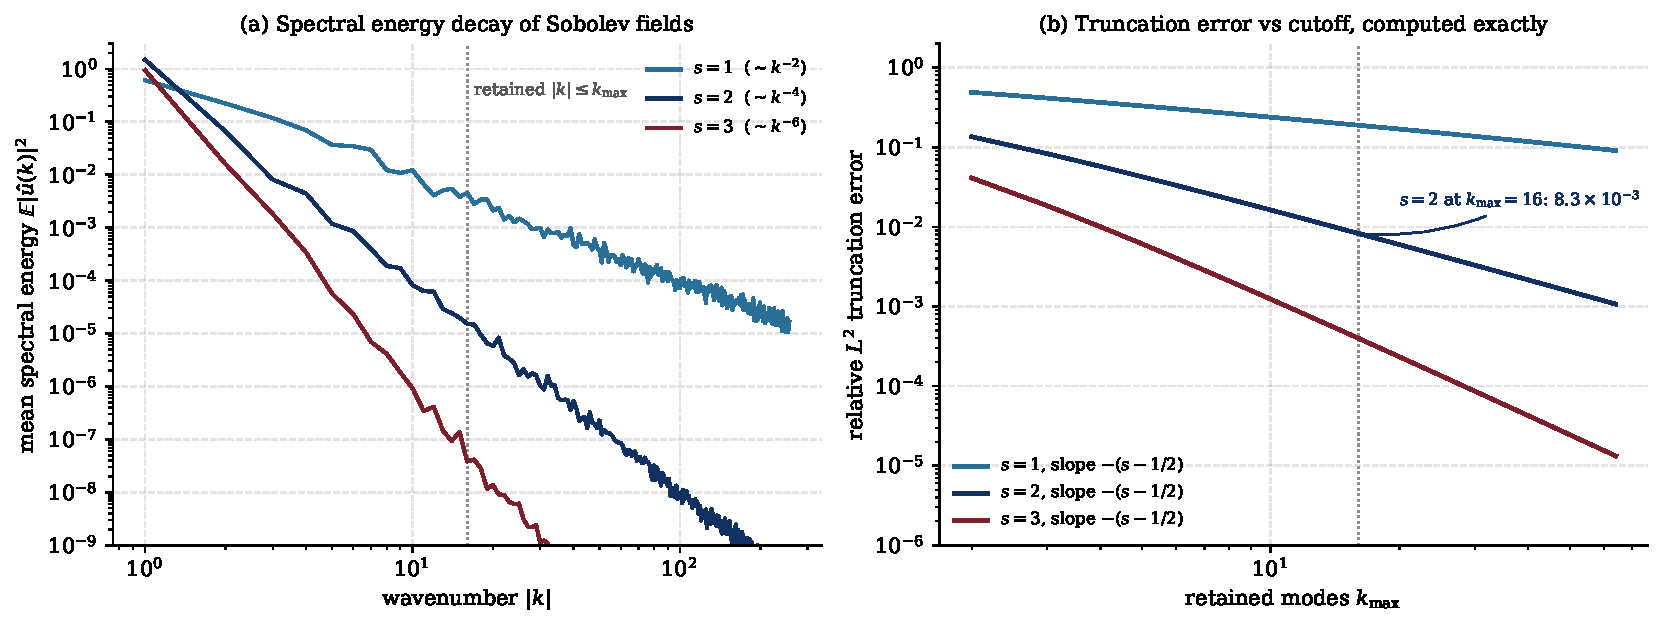
\includegraphics[width=0.88\textwidth]{fig_spectral_decay.pdf}
\caption{\textbf{Spectral decay and the cost of truncation, computed rather than drawn schematically.} Both panels use the Sobolev model $\hat{u}(k) = |k|^{-s}\xi_k$ with $\xi_k$ independent standard normal and $s \in \{1,2,3\}$. (a) Mean spectral energy $\mathbb{E}|\hat{u}(k)|^2 = k^{-2s}$, averaged over 40 draws, with the dotted vertical line marking a retained band $|k| \le k_{\max} = 16$. (b) Exactly computed relative $L^2$ error of the band projection $P_{k_{\max}}$ of \eqref{eq:ch05-projection}, namely $\|(I-P_{k_{\max}})u\|_{L^2}/\|u\|_{L^2} = \big(\sum_{k_{\max}<k\le 512} k^{-2s} \big/ \sum_{1\le k\le 512} k^{-2s}\big)^{1/2}$ on a grid resolving $|k| \le 512$, for $k_{\max} = 2,\dots,64$; the log-log slope is $-(s-\tfrac12)$, as marked. Panel (b) isolates truncation: no horizontal line is drawn, because the neural term of \eqref{eq:ch05-error-decomposition} is measured for exactly one
architecture in this book, the worked example of Appendix~\ref{app:b}, and its value belongs in
that appendix rather than on this axis. The dotted vertical line marks an illustrative cutoff, $k_{\max}=16$; the worked example of Appendix~\ref{app:b} retains $k_{\max}=11$. That example is the one-dimensional periodic heat equation $u_t = \alpha u_{xx}$ with $\alpha = 0.01$ at $T = 1$, trained on inputs $u_0(x) = \sum_{k=1}^{8} c_k k^{-3/2}\cos(2\pi k x + \phi_k)$ with $c_k \sim \mathcal{N}(0,1)$ and $\phi_k$ uniform on $[0,2\pi)$, whose exact solution is $u(x,T) = \mathcal{F}^{-1}\!\big[\hat{u}_0(k)\,e^{-\alpha(2\pi k)^2 T}\big]$. The callout is the computed value at $k_{\max}=16$ for $s=2$, $8.3\times10^{-3}$, at the same cutoff drawn in panel (a). A curve that has fallen far below it is not thereby accurate --- only no longer limited by truncation.}
\label{fig:spectral_decay}
\end{figure}

Figure~\ref{fig:spectral_decay} is what a practitioner should take from
Theorem~\ref{thm:fno_convergence}. Panel (a) shows the energy bookkeeping that
makes \eqref{eq:ch05-modeset} defensible: the tail beyond a moderate cutoff
carries a small and rapidly shrinking share of the total, and the share shrinks
faster the larger the regularity $s$, which is \eqref{eq:ch05-coefficient-decay}
summed in $\ell^2$. Panel (b) converts that bookkeeping into the accuracy the
reader can expect from the first term of \eqref{eq:ch05-error-decomposition}.
Doubling $k_{\max}$ divides the relative truncation error by the asymptotic
factor $2^{\,s-1/2}$ --- $1.4$ at $s=1$, $2.8$ at $s=2$, $5.7$ at $s=3$ --- and
the computed curves come close to it: between the cutoffs $k_{\max} = 32$ and
$k_{\max} = 64$ the observed factors are $1.46$, $2.80$ and $5.55$. At the band
$k_{\max} = 16$ drawn in panel (a), the computed error is $8.3\times10^{-3}$ for
$s=2$, against $1.9\times10^{-1}$ at $s=1$, which has fallen only to
$9.1\times10^{-2}$ by the largest cutoff plotted. At one band the two curves are a
factor of $23$ apart, and what separates them is regularity. Two conclusions
follow. Once the algebraic curve has fallen below the
network's own term, adding modes buys nothing: the second term of
\eqref{eq:ch05-error-decomposition} dominates, and where that crossing sits is a
property of a particular training run. That is why the
one-dimensional example of Appendix~\ref{app:b} and the two-dimensional
reference configuration of \chapref{ch:part2-fourier-neural-operators-fno-from-scratch}
keep of order a dozen to sixteen modes per direction, not hundreds. And a
target with only one derivative is not rescued by any affordable mode budget:
regularity, not resolution, is the binding constraint.

The model problem in the caption also marks the boundary of the argument's
honesty. Heat diffusion multiplies mode $k$ by $e^{-\alpha(2\pi k)^2 T}$, which
at $\alpha = 0.01$, $T = 1$ is $1.1\times10^{-11}$ already at $k = 8$: the
solution operator smooths far faster than any power, so its truncation term is
negligible and the observed error is entirely $\mathcal{E}_{\text{NN}}$. That is
a property of the example, not a general guarantee, and the linear heat equation
is an easy case for any classical solver; the surrogate there is a teaching
device. The bound \eqref{eq:ch05-error-decomposition} earns its keep on
nonlinear targets that smooth without being analytic, and it weakens exactly
where the hypothesis of Theorem~\ref{thm:fno_convergence} fails.
\index{heat equation!spectral damping of the solution operator}

\takeaway{What the Mode Budget Buys}{For a target gaining $\alpha$ derivatives,
the truncation term of \eqref{eq:ch05-error-decomposition} is algebraic in
$k_{\max}$ and independent of depth, width, and grid; the capacity term
$\mathcal{E}_{\text{NN}}(L,d_v)$ is the part the theory can drive small but not
rate. The two set each other's useful range, and nothing in the bound connects
either of them to sample size or to the optimizer.}

\medskip
Where the argument stops, the next chapter begins.
Theorem~\ref{thm:fno_convergence} bounds the distance between a target operator
and a continuum FNO whose layer \eqref{eq:fno_layer} is written with continuous
transforms $\mathcal{F}$, $\mathcal{F}^{-1}$; a real network never computes
those. It evaluates coefficient sums on $N$ grid points, where the FFT replaces
$\mathcal{F}$ with a discrete transform whose coefficients are quadrature
approximations carrying aliasing of their own. Nothing in
\eqref{eq:ch05-error-decomposition} mentions a grid --- and that is the whole
point of the chapter that follows. The theorem bounds a continuum object, so
what still requires proof is a commutation of limits, not a property of $C_1$
or of $\mathcal{E}_{\text{NN}}$: that the discrete operator induced by any grid
converges to the continuum operator as $h \to 0$, and that the parameter vector
$\phi$ means the same object on every grid. \chapref{ch:part1-discretization-invariance-and-continuum-li} states that
property precisely, checks it for the spectral layer against the quadrature
consistency of the generic kernel, and shows why a conventional convolutional
network fails the same test --- with a consequence, zero-shot evaluation on
finer grids, that follows from the fixed band \eqref{eq:ch05-modeset} as soon as
the input is resolved on the training grid.
